\chapter*{Prefácio}
\addcontentsline{toc}{chapter}{Prefácio}
\chaptermark{Prefácio}
\epigraph{``\textit{Any fool can write code that a computer can understand. Good programmers write code that humans can understand}''.}{Martin Fowler}

\lettrine[lines=4, lhang=0.1, lraise=0, loversize=0.2, findent=0.1em]{\textcolor{corTema}{P}}{rezado} leitor, seja bem-vindo! Os Capítulos deste livro foram organizados de forma a guiá-lo no processo de fixação dos conteúdos aprendidos durante a sua leitura por meio de exercícios, desafios e de projetos práticos aplicados no contexto de desenvolvimento de aplicações Web em Java e outras tecnologias. A ordem dos Capítulos obedece a um caminho lógico que será empregado para auxiliá-lo no processo de aprendizagem das tecnologias e técnicas discutidas, ou seja, a organização dos Capítulos segue a ordem cronológica dos tópicos que serão apresentados, ensinados e treinados.

\begin{wrapfigure}{R}{0.3\textwidth}
    \centering
    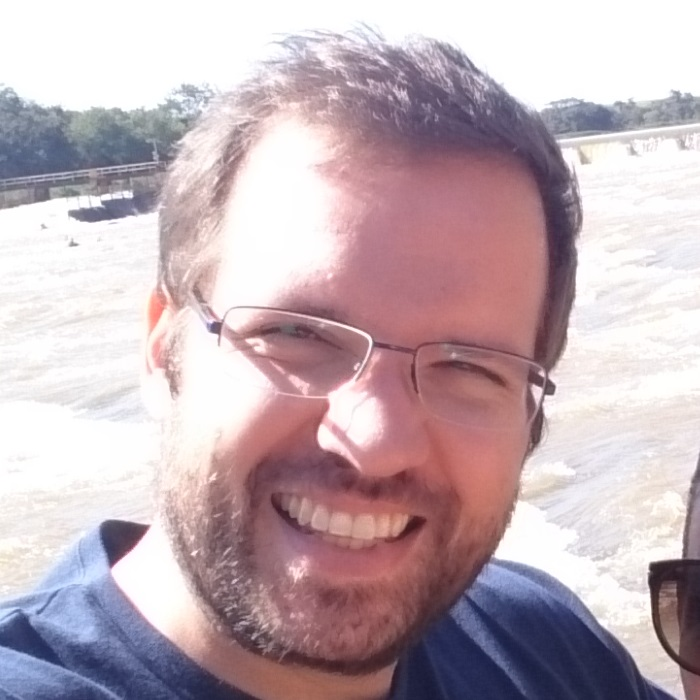
\includegraphics[width=0.25\textwidth]{imagens/david}
\end{wrapfigure}

Antes de começar, eu gostaria de me apresentar. Meu nome é David Buzatto e sou Bacharel em Sistemas de Informação pela Fundação de Ensino Octávio Bastos (2007), Mestre em Ciência da Computação pela Universidade Federal de São Carlos (2010) e Doutor em Biotecnologia pela Universidade de Ribeirão Preto (2017). Atualmente meus principais interesses giram em torno de temas relacionados à construção de compiladores, teoria da computação, análise e projeto de algoritmos, estruturas de dados, algoritmos em bioinformática e desenvolvimento de jogos eletrônicos. Atualmente sou professor efetivo do Instituto Federal de Educação, Ciência e Tecnologia de São Paulo (IFSP), câmpus São João da Boa Vista. A melhor forma de contatar é através do e-mail \textcolor{corTema}{\href{mailto:davidbuzatto@ifsp.edu.br}{davidbuzatto@ifsp.edu.br}}.

Para que você possa aproveitar a leitura deste livro de forma plena, vale a pena entender alguns padrões que serão utilizados neste texto. As quatro caixas apresentadas abaixo serão empregadas para mostrar, a você leitor, respectivamente, boas práticas de programação, conteúdos complementares para melhorar e aprofundar seu aprendizado, observações pertinentes ao que está sendo apresentado e, por fim, itens que precisam ser tratados com cuidado ou que podem acarretar em erros comuns de programação.

\begin{boaPratica}
    Essa é uma caixa de ``Boa Prática''.
\end{boaPratica}

\begin{saibaMais}
    Essa é uma caixa de ``Saiba Mais''.
\end{saibaMais}

\begin{observacao}
    Essa é uma caixa de ``Observação''.
\end{observacao}

\begin{atencao}
    Essa é uma caixa de ``Atenção!''.
\end{atencao}

Você notará que este este livro foi escrito de forma quase coloquial, com o objetivo de conversar com você e não com o objetivo de ser um material de pesquisa. É de suma importância que você procure implementar os exemplos apresentados e que resolva cada um dos exercícios básicos de cada Capítulo, visto que a utilização de uma linguagem de programação ou tecnologia, e mais importante ainda, a obtenção de maturidade no desenvolvimento de \textit{software}, é ferramenta primordial para o seu sucesso profissional e intelectual.

Vale ressaltar que este livro e os projetos apresentados serão constantemente atualizados, sendo assim, sempre obtenha as últimas versões dos mesmos \textcolor{corTema}{\href{https://github.com/davidbuzatto/Livro-Desenvolvimento-de-Aplicacoes-Web-em-Java/releases}{aqui}}. Espero que essa obra, de distribuição totalmente gratuita, lhe seja útil!
    

\vspace*{\fill}
